\chapter{Sprint 2}
	
\section*{Introduction}
   In this Sprint we go through the planning, analyzing, and implementing phases of the Employee module.\\
   At the beginning of this sprint, we held a second planning meeting where we set the following objectives:

\begin{itemize}
\item This sprint is spread over Three weeks.
\item At the end of this sprint the employee module will be delivered
\item Development of the sprint2 Backlog
\item Elaboration of a design phase
\end{itemize}
\\
This second iteration of our project's lifecycle encompasses the design, development and implementation of the Employee Managment module developed around the Odoo ERP base hr.employee model
\section{Sprint backlog}
The following table summarizes the tasks that we are responsible for carrying out 
\begin{center}
\begin{longtable}{|p{1cm}|p{6,25cm}|p{0,7cm}|p{6,25cm}|p{0,8cm}|}
\caption{ Project backlog }
\hline
\textbf{US ID} 
&\textbf{User Story}
&\textbf{T ID}
&\textbf{Task}
&\textbf{Esti- ma- tion}
\\
\hline
\multirow{ 3}{*}{0}
&\multirow{3}{*}{Storyless}
&0.1
&Class diagram
&4h\\\cline{3-5}
&
&0.2
&Use case diagram
&8h\\\cline{3-5}
&
&0.3
&Documenting progress
&2h\\\cline{3-5}
\hline
\multirow{2}{*}{2}
&\multirow{2}{=}{As an Administrator, I want to be able to create user accounts}
&2.1
&Create the «Employee» model
&8h\\\cline{3-5}
&
&2.2
&Link «Employee» model to Odoo user account
&8h\\\cline{3-5}

\hline
3
&As an Administrator, I want to be able to edit user details
&3.1
&Create «Employee» model security rules
&1h
\\\hline


\multirow{ 2}{*}{4}
&\multirow{2}{=}{As a Manager, I want to be able to edit user roles}
&4.1
&Define our user groups
&2h\\\cline{3-5}
&
&4.2
&Add the user groups to security file
&8h\\\cline{3-5}
\hline


\multirow{ 4}{*}{5}
&\multirow{4}{=}{As an Administrator, I want to be able to view the users list}
&5.1
&Create the «All Employees» view
&8h\\\cline{3-5}
&
&5.2
&Add search and filter actions
&4h\\\cline{3-5}
&
&5.3
&Create security rules
&1h\\\cline{3-5}
&
&5.4
&Create the «Users» menu item
&30m\\\cline{3-5}

\hline


\multirow{4}{*}{6}
&\multirow{4}{=}{As a User , I want to be able to view my profile details}
&6.1
&Create the «Employee» view
&16h\\\cline{3-5}
&
&6.2
&Create the «vaccine\_record» model
&4h\\\cline{3-5}
&
&6.3
&Create the «visa\_record» model
&4h\\\cline{3-5}
&
&6.4
&Add related models to the view
&6h\\\cline{3-5}

\hline

\multirow{2}{*}{7}
&\multirow{2}{=}{As a User , I want to be able to change my profile details}
&7.1
&Create model security rules
&1h\\\cline{3-5}
&
&7.2
&Change the editable attribute on desired fields
&2h\\\cline{3-5}

\hline
\end{longtable}
\end{center}
\section{Software Design}
The conceptual study conducted at the beginning of an iteration allows us to evaluate the sprint in its early stages by providing a stable reference of conceptual data model and processing to identify potential scenarios.

        \subsection{Use case diagram}
    \begin{figure}[H]
    \begin{center}
        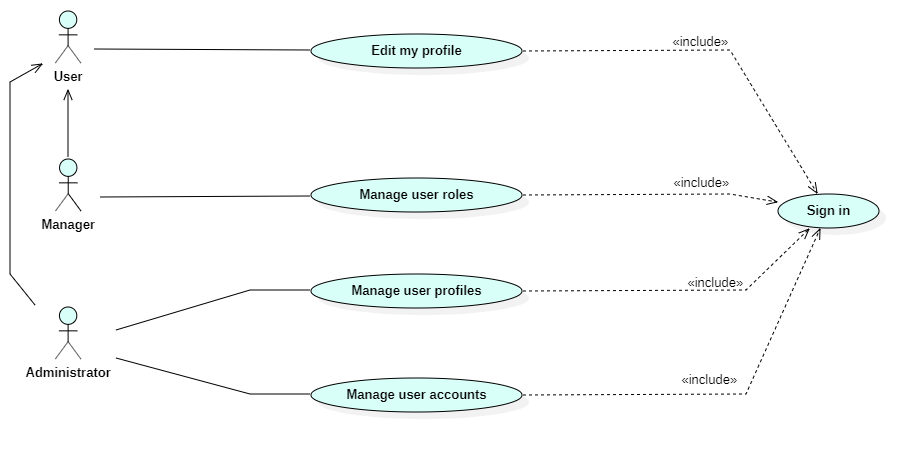
\includegraphics[scale=0.4]{img/sprint2_usecase.png}
        \caption{Sprint 2 use case diagram}
    \end{center}
     \label{fig:my_label}
\end{figure}

    \subsection{Class diagram}
        \begin{figure}[H]
    \begin{center}
        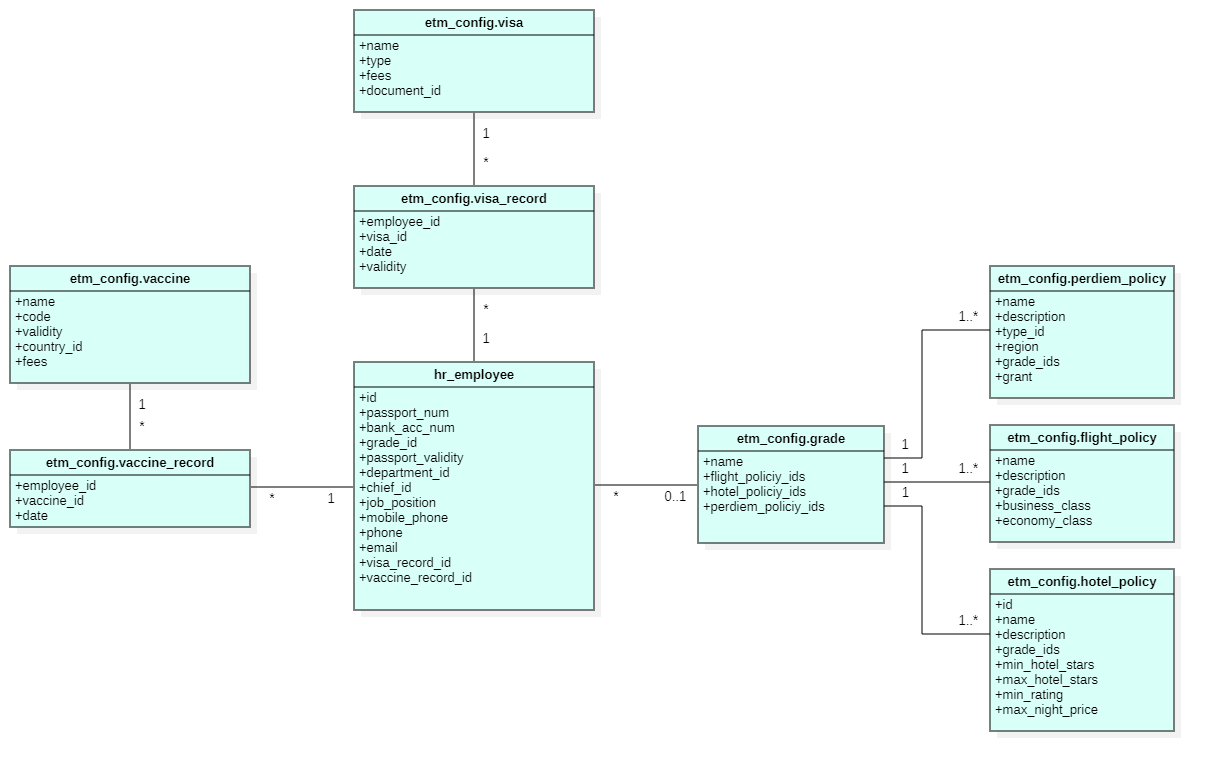
\includegraphics[scale=0.42]{img/sprint2_class.png}
        \caption{Sprint 2 class diagram}
    \end{center}
     \label{fig:my_label}
\end{figure}
        

In this section we will present the refinement of some use cases as well as the sequence diagram. 

\subsection*{Use case «Edit my profile»}
\begin{figure}[H]
    \begin{center}
        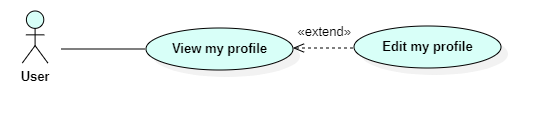
\includegraphics[scale=0.6]{img/sprint2_edit_profile_usecase.png}
        \caption{«Edit my profile» detailed use case diagram}
    \end{center}
        \label{fig:my_label}
\end{figure} 
    The following table addresses the use case previously illustrated by providing a textual description, post and preconditions as well as the main scenario and the nominal scenario
    \begin{center}
    
\begin{longtable}{|p{4,25cm}|p{9,25cm}|}
\caption{«Edit my profile» detailed textual description}
\hline
\textbf{Use Case}&Edit my profile
\\\hline
\textbf{Actors}&User
\hline
\textbf{Pre-condition}&User signed in and viewing profile
\hline
\textbf{Post-condition}&Profile edited
\hline
\textbf{Basic path}&
        \begin{enumerate}
         \item The user clicks on the button "Edit"
         \item The system displays a form containing current information
         \item The user edits the information
         \item The user clicks on the button "Save"
         \item The system processes the input
         \item The system saves the new information
         \item The user is sent back to the profile view
     \end{enumerate}\\
\hline
\textbf{Alternative path}&
\begin{itemize}
\item 4.Duplicate or missing Data (The user is sent back to step 2)
\item 4.No changes were made (The system skips to step 7)
\end{itemize}\\
\hline
\end{longtable}
\end{center}




\subsection*{Use case «Manage user roles»}
\begin{figure}[H]
    \begin{center}
        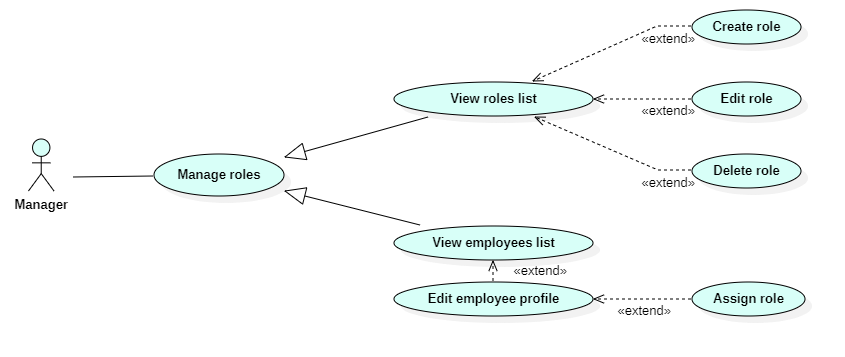
\includegraphics[scale=0.6]{img/sprint2_manage_roles_usecase.png}
        \caption{«Manage user roles» detailed use case diagram}
    \end{center}
        \label{fig:my_label}
\end{figure} 
    The following tables addresses the «Edit employee profile» use case detailing access and edit rights for each actor\\
    
\begin{center}
\begin{longtable}{|p{6,25cm}|p{1,5cm}|p{1,5cm}|p{1,5cm}|}
\caption{«User profile» access right}
\hline
&User&Manager&Admin
\\\hline
Can view user list&Yes&Yes&Yes
\hline
Can view user public information&Yes&Yes&Yes
\hline
Can view user private information&No&Yes&Yes
\hline
Can view user policies&No&Yes&Yes
\hline
Can view user Visa and vaccine history&No&Yes&Yes
\hline

\end{longtable}
\end{center}
\newpage
\begin{center}
\begin{longtable}{|p{6,25cm}|p{1,5cm}|p{1,5cm}|p{1,5cm}|}
\caption{«User profile» edit right}
\hline
&User&Manager&Admin
\hline
Can edit own profile&Yes&Yes&Yes
\hline
Can edit other's profile&No&Yes&Yes
\hline
Can edit other's private information&No&No&Yes
\hline
Can edit other's public information&No&No&Yes
\hline
Can assign policies&No&Yes&Yes
\hline
Can assign roles&No&Yes&Yes
\hline
Can edit visa and vaccine history&No&No&Yes
\hline
\end{longtable}
\end{center}





\subsection*{Use case «Manage user profiles»}
\begin{figure}[H]
    \begin{center}
        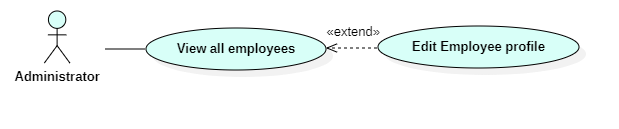
\includegraphics[scale=0.6]{img/sprint2_admin_edit_profile_usecase.png}
        \caption{«Manage user profiles» detailed use case diagram}
    \end{center}
        \label{fig:my_label}
\end{figure} 

The Administrator has the right to edit all fields of the user profile, these fields are split into categories. the table below will list all fields and their respective categories:\\
\newpage
\begin{center}
\begin{longtable}{|p{4,25cm}|p{9,25cm}|}
\caption{«Employee profile» fields list}
\hline
\textbf{Public information}&
\begin{itemize}
\item Full name
\item Phone
\item Mobile phone
\item Department
\item Job Position
\item Hierarchical Chief
\end{itemize}
\hline
\textbf{Private information}&
\begin{itemize}
\item Identifier
\item Bank account number
\item Passport number
\item Passport validity
\end{itemize}
\hline
\textbf{Policies}&
\begin{itemize}
\item Flight policy
\item Hotel reservation policy
\item Per Diem policy
\end{itemize}
\hline
\textbf{Grade}&Grade
\hline
\end{longtable}
\end{center}



\subsection*{Use case «Manage user accounts»}
\begin{figure}[H]
    \begin{center}
        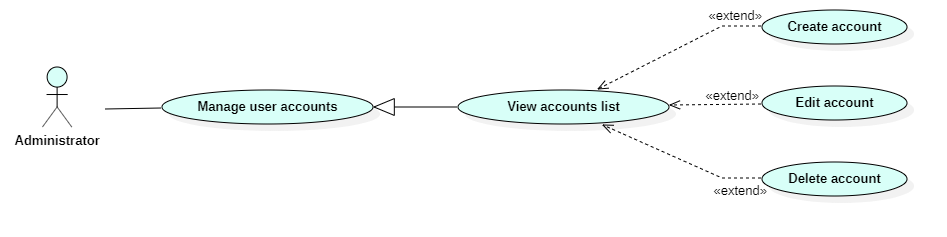
\includegraphics[scale=0.55]{img/sprint2_manage_accounts_usecase.png}
        \caption{«Manage user accounts» detailed use case diagram}
    \end{center}
        \label{fig:my_label}
\end{figure} 

\begin{center}
\begin{longtable}{|p{4,25cm}|p{9,25cm}|}
\caption{«Create account» detailed textual description}
\hline
\textbf{Use Case}&Create account
\\\hline
\textbf{Actors}&Administrator
\hline
\textbf{Pre-condition}&Administrator signed in and viewing account list
\hline
\textbf{Post-condition}&Account created
\hline
\textbf{Basic path}&
        \begin{enumerate}
         \item The Administrator clicks on the button "Create"
         \item The system displays a a empty form
         \item The Administrator fills the form
         \item The Administrator clicks on the button "Save"
         \item The system processes the input
         \item The system creates a new account
         \item The Administrator is sent back to the account list view
     \end{enumerate}\\
\hline
\textbf{Alternative path}&
\begin{itemize}
\item 4.Duplicate or missing Data (The Administrator is sent back to step 2)
\item 2.Administrator clicks on the button "Cancel"(System skips to step 7)
\end{itemize}\\
\hline
\end{longtable}
\end{center}



\section{Implementation}
This section presents some user interfaces of the module with screenshots to further clarify our work. The figures below present these interfaces, starting with the first figure which shows the Employee list view , in this view we can access any employee file or create new employees

\begin{figure}[H]
    \centering
    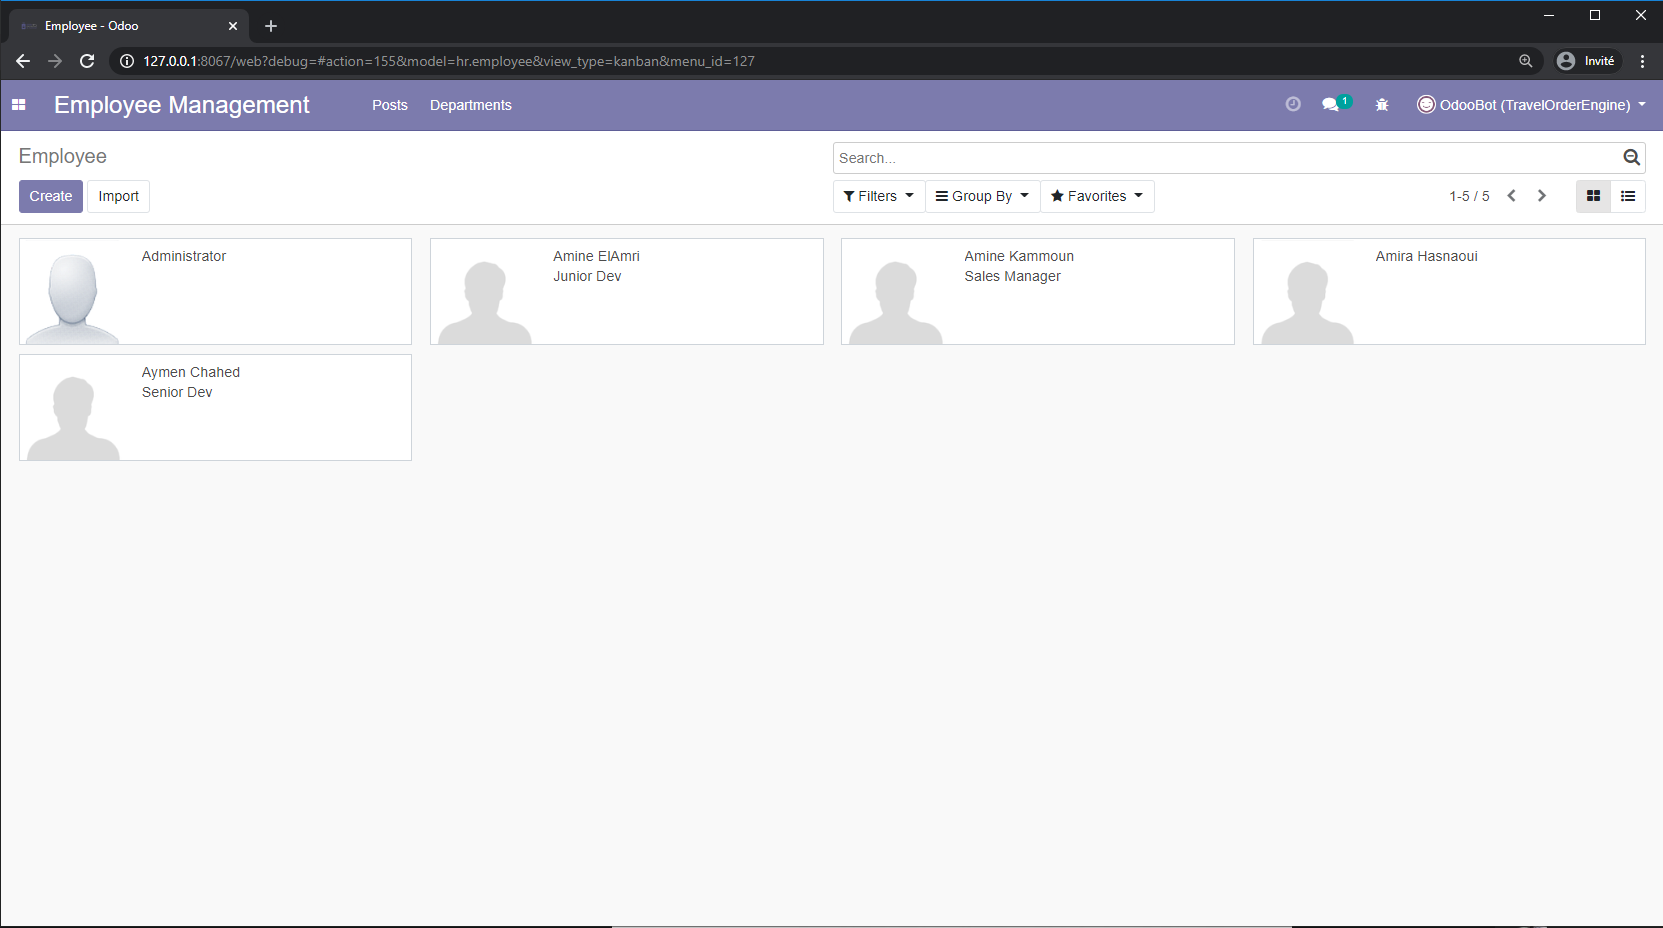
\includegraphics[scale=0.38]{img/c_employees.png}
    \caption{Employees list view}
    \label{fig:my_label}
\end{figure}

In this figure we will show the Employee view, All the employee information is displayed here . it is the same form we use for creating employees. The administrator can edit all the information by clicking the "Edit" button above
\begin{figure}[H]
    \centering
    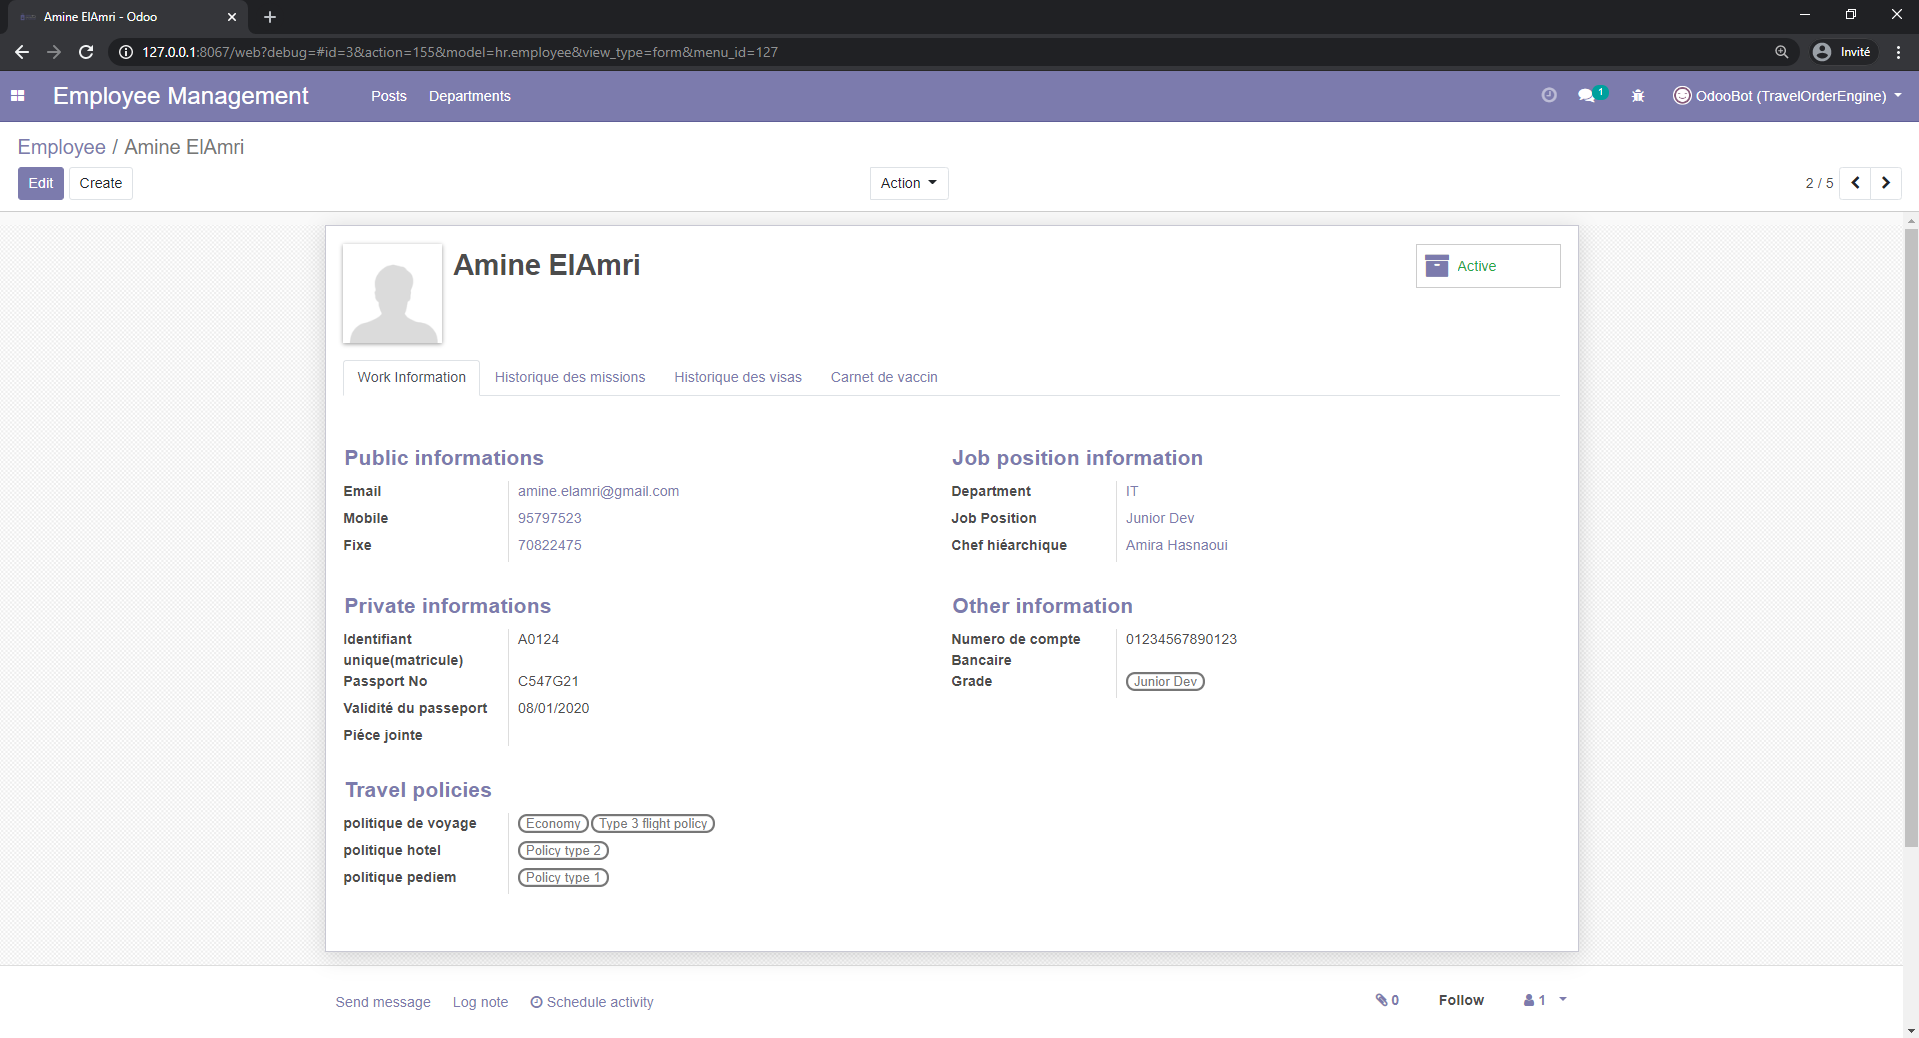
\includegraphics[scale=0.33]{img/c_employee.png}
    \caption{Employee view}
    \label{fig:my_label}
\end{figure}
In this figure we will show the Department list view, here we can create and edit the departments and set the department's manager.
\begin{figure}[H]
    \centering
    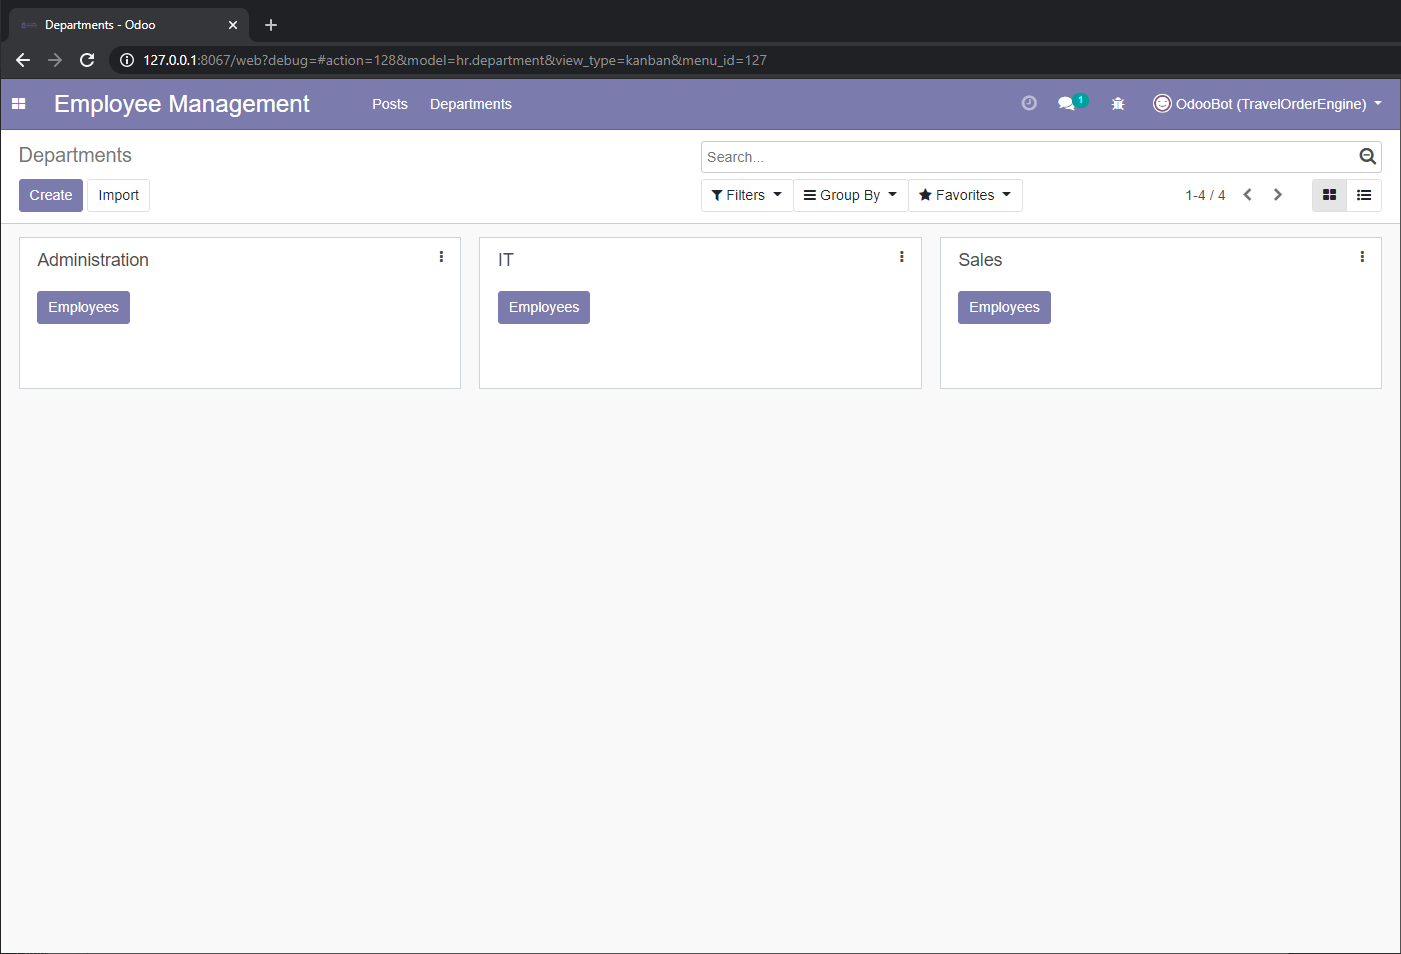
\includegraphics[scale=0.44]{img/c_departements.png}
    \caption{Departments list view}
    \label{fig:my_label}
\end{figure}
In this last figure we will show the job positions list view , Administrator can add or edit jobs on this list, Employees can have only 1 job position at a time.
\begin{figure}[H]
    \centering
    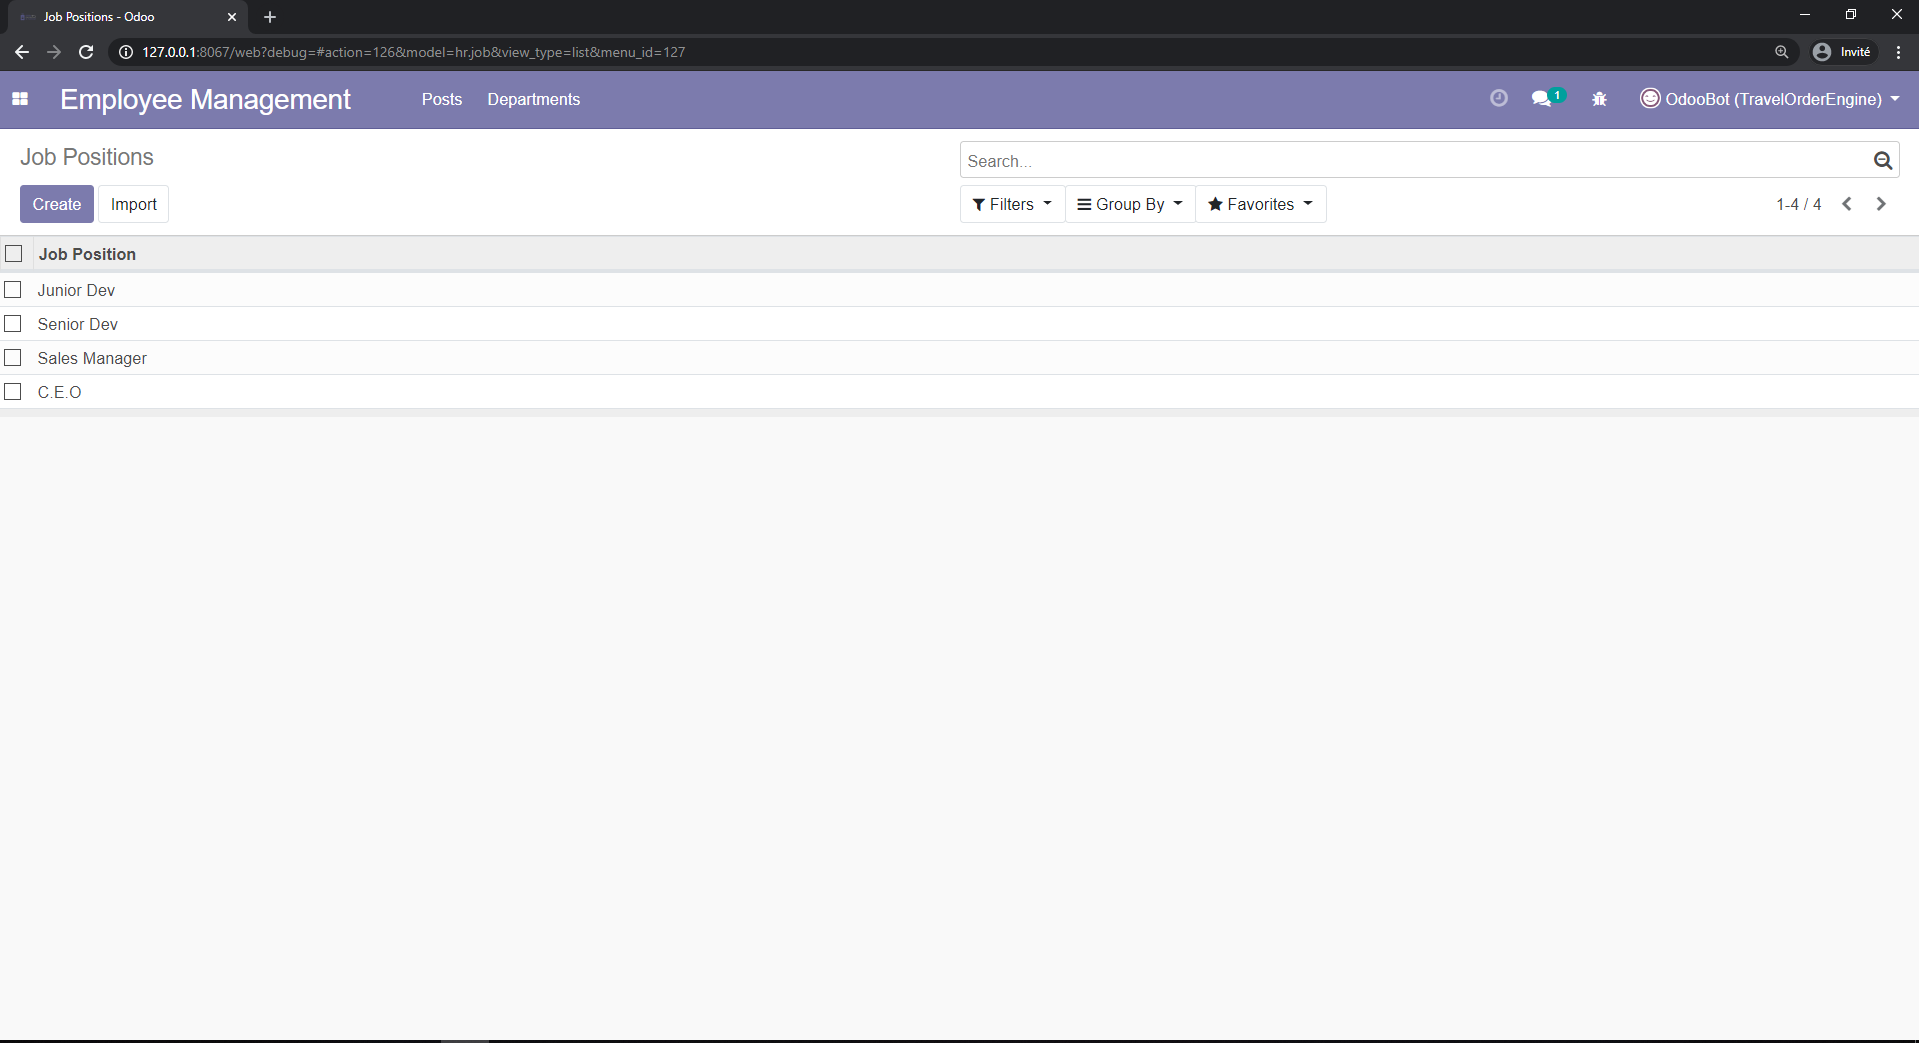
\includegraphics[scale=0.32]{img/c_jobs.png}
    \caption{Job positions list view}
    \label{fig:my_label}
\end{figure}





\section*{Conclusion}
  This chapter covered the sprint2 of our project. We started by explaining the objective of this sprint and the main actors. Then we presented our Sprint2 backlog. We continued with the design phase where we schematized some design diagrams in UML and we closed the chapter by exposing the interfaces of the second increment.  \\ 
In the following, we will address the last sprint of this project which will involve the design, development, and implementation of the travel order management module.